\section*{Motivation}

%%<why do opvs matter>
The global climate crisis is one of the most pressing issue humanity faces today.
\begin{wrapfigure}{l}{0.5\linewidth}
    \centering
    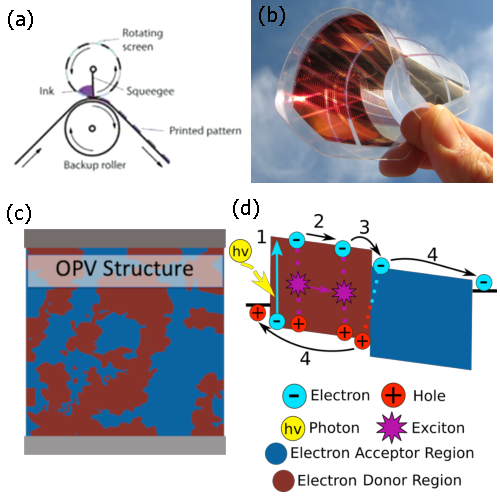
\includegraphics[width=\linewidth]{images/dou-miller2018c-fig.pdf}
    \caption{Schematic showing (a) roll to roll printing process for OPVs, (b) example OPV device, (c) bulk heterojunction structure, and (d) OPV energy generation process. Part (a) adapted from ref \cite{Dou2013}. Parts (b)-(d) adapted from ref \cite{Miller2018c}.}
    \label{fig:opv}
\end{wrapfigure}
Consumption of fossil fuels for energy and transportation strongly contributes to atmospheric $CO_2$ the affects of which are global, long-term, and devastating\cite{Solomon2009a}.
%% should I put examples? fires https://science2017.globalchange.gov/chapter/8/
In our technology-driven society, it is unrealistic to think that energy demand will lessen, in fact global energy consumption is predicted to increase from 17 TW in 2010 to 27 TW in 2040\cite{Mazzio2015}.
In order to protect our climate, we need a non-polluting, cost-efficient way to provide electricity.
Harnessing solar energy is an important part of a green energy solution.
Renewable energy accounted for 11\% of the U.S. energy consumption in 2019 and of that 9\% was from solar (solar accounted for approximately 1\% of the total energy)\cite{USEIA2020}.
Our energy infrastructure has room for improvement: consider Germany which in 2019 got 43\% of its energy from renewables and 8.2\% of its total energy from solar\cite{Wirth2017}.
Traditionally, photovoltaic devices, which can convert incedent light into electric current, were made of inorganic materials like silicon.
But in the late 1970's organic photovaltaics (OPVs) were discovered as a potential alternative\cite{Tang1986b}.
The advantage of OPVs over inorganic PV devices is that OPVs are lightweight, low cost, easier to produce, and flexible. 
OPVs can be manufactured large scale in a roll to roll printing process, similar to newspaper as shown in \autoref{fig:opv} a\cite{Dou2013}.
However, other materials still outperform OPVs (see Figure \ref{fig:nrel}) and in order to become a viable, cost-effective option OPVs need to be more efficient\cite{Mazzio2015}.

\begin{figure}[h!]
    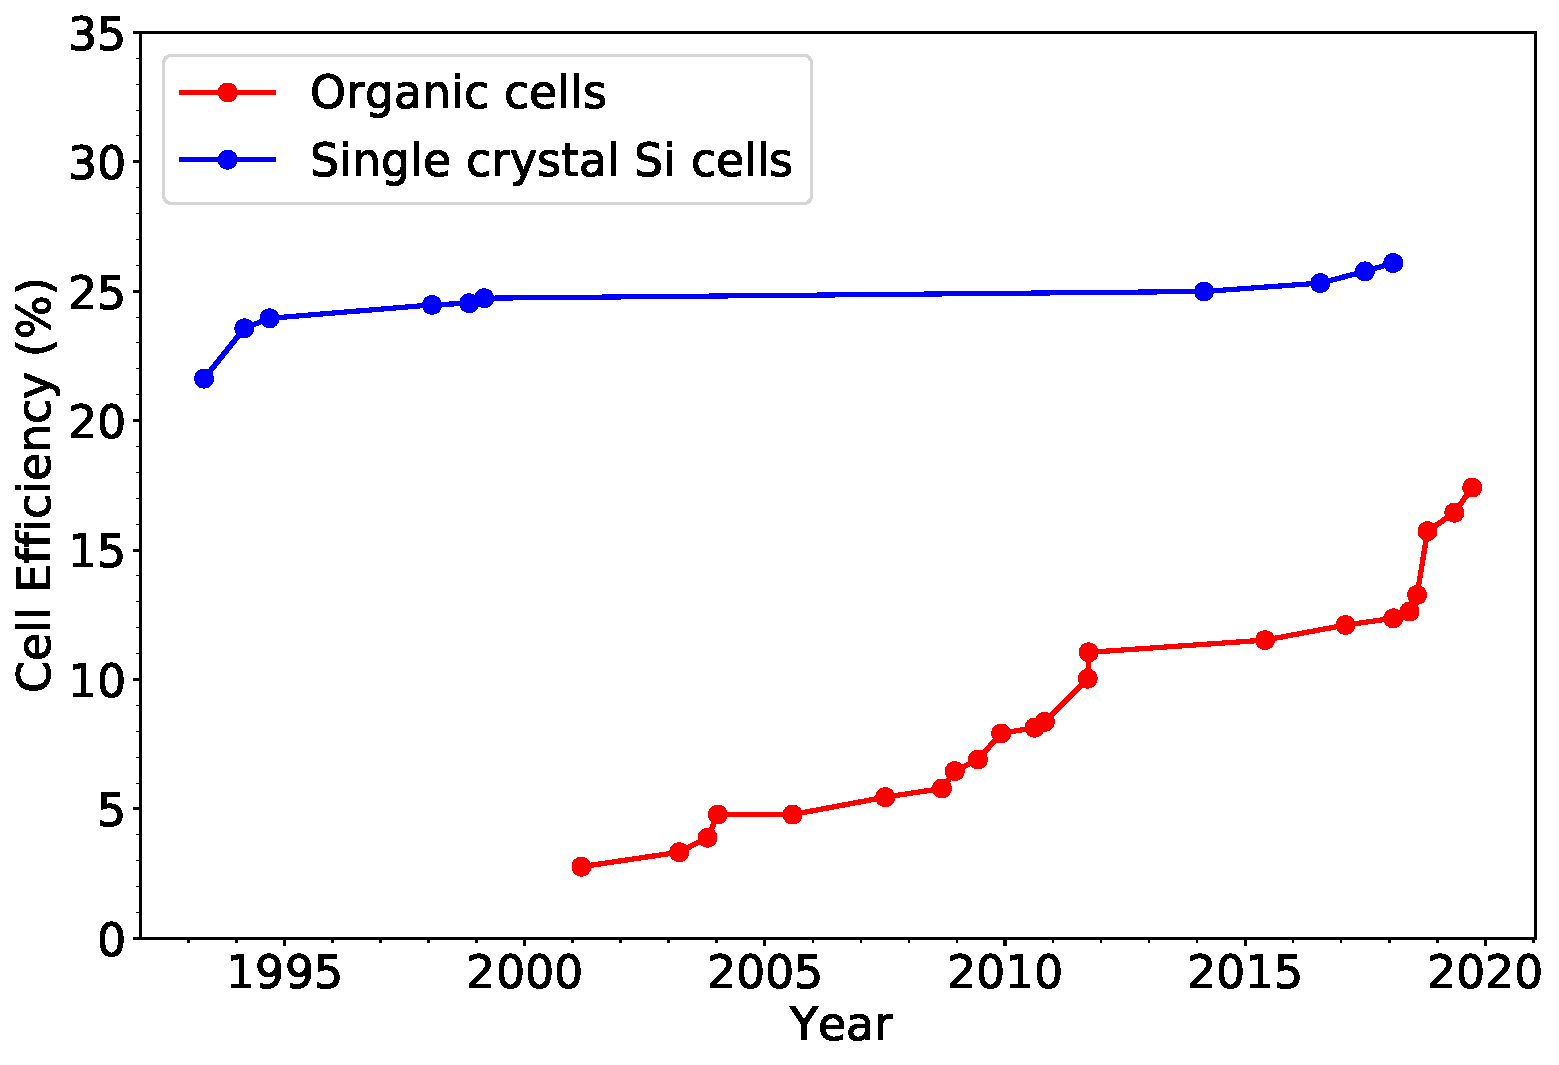
\includegraphics[width=0.9\linewidth]{images/NREL2020.pdf}
    \caption{Efficiencies of all photovoltaic technologies from 1976 to present. OPVs are denoted by red filled circles. The current state-of-the-art OPV research cell achieves 17.4\% efficiency. Image taken from ref \cite{NREL2020}.}
    \label{fig:nrel}
\end{figure}
\cite{Cui2019}
%% new figure
%% TODO
%% opvs are vast
%% crystalline silicon levels off -- shottkey quessar (sp?) limit 34% efficient not much room for growth (blue)
%% what you can buy vs champion devices
%% opvs show room to grow
%% paying for themselves
%%underdog
In order to make the most efficient OPVs we need to find the blend of compounds and processing conditions that result in the best structure for those compounds.
The active layer of an OPV is mixture of electron-donor and acceptor compounds: the ideal morphology is a micro phase-separated interpenetrating network called a bulk heterojunction (BHJ) (see Figure \ref{fig:opv} c).
The performance of an OPV device is intimately linked with the structure of the active layer:
With minor modifications, the number of compounds and the processing conditions can become infinite which makes this an intractable problem for experiment.

% TODO
%% include fig of ITIC PTB7? p3ht, fullerene recent uptick with NFAs
%% look up the 17% solar cell--whats in it?
%% freedom in choosing our ingredients - can we get better than trial and error
\cite{Cui2019}
chlorinated ladder backbone acceptor 16\% PCE 
%% https://www.printedelectronicsworld.com/articles/15405/raynergy-new-world-record-on-certified-pce-13-28-single-junction-opv
signle junction with NFA

Imagine, you are a chemist synthesizing and testing new OPV morphologies: you are specifically looking at a mixture of a non-fullerene acceptor, ITIC, and a polymer donor, PTB7. 
Each compound costs \$500 for 100 mg\cite{sigmaaldrich}.
The solvent you use and the concentrations of your active compounds changes the device performance\cite{Hoppe2004a}.
The amount of time the solvent is allowed to evaporate changes the device performance\cite{Li2007}.
The time and temperature of the thermal annealing changes the device performance\cite{Ma2005}.
The regioregularity of your polymer affects the device performance\cite{Kim2006}.
The distribution of polymer lengths affects the device performance\cite{Zhao2013b}.
Changing the functional groups on ITIC changes how it packs in a crystal, its electron affinity, and thus its performance in a device\cite{Swick2019a}.
All this would be to determine the performance of just one donor/acceptor combination in one category of potential compounds\cite{Dou2013}.
This is where molecular simulation can help.
By using a simulation pipeline, we can help to streamline the process of determining which OPV materials will form the best morphology with the best charge transport, and in turn, help to solve the energy crisis.

Molecular simulation also gives us insight into the atomic interactions which drive the self assembly of an OPV morphology.
A complication of the simulation of OPV polymers is that the properties which predict a device's efficiency, for example charge transport, span multiple length scales.
The atomic and electronic properties are important for light absorption, in which an exciton is created, and charge transfer, where the exciton is dissociated into a free electron and hole\cite{Scharber2006a,Hoppe2004,Mazzio2015}.
At the same time, the exciton finding an interface at which to dissociates depends on the bulk morphology, as do the charges, once separated, finding a path to an electrode in order to generate current and produce electricity.
So, in order to model this system, a multiscale approach is necessary.
By breaking our simulation apart into separate steps and equilibrating different lengths scales individually, we can get equilibrated morphologies on multiple length scales more efficiently.

Already good open-source packages exist to address the problem of coarse-graining and/or backmapping\cite{Marrink2007,Ruhle2009,Maerzke2011,MorphCT,Wassenaar2014b}. %%these citations are martini, votca, trappe, morphct, backwards.py
By making code open source and freely availiable, we contribute to the knowledge of a global community. 
But just because something is availiable doesn't mean it is accessible: often just figuring out how to use an existing package can be very difficult\cite{Cummings2019}.
These existing codebases can appear to a new user as monolithic and indecipherable because their design has been to solve a problem, which they do, instead of design with a focus on how people learn.
These codebases also rely on users piecing together multiple, often incompatible, bits of software, using manually created xml files, or deciding how to classify an atom grouping based on the user's chemical intuition.
All of these factors contribute to a reproducibility crisis in the computational sciences\cite{Baker2016}.
By keeping best practices for software development and teaching in mind throughout development, we can strive to make tools which make science more transferrable, reproducibile, usable, and extensible (TRUE)\cite{Thompson2020}. %%TRUE
Best software development practices include using version control software, such as git, to facilitate the process of tracking and merging changes to a code repository, especially important when working collaboratively.
Also among these best practices are using unit tests and continuous integration to ensure that errors are quickly and automatically caught\cite{Wilson2014}.
Instead of writing dense, inseparable scripts which rely on the user manually following a command prompt or editing multiple text files, we aim to keep code small and modular to make it easier to use and understand\cite{Adorf2018a}.
Following these guidelines not only makes our code easier to develop and debug but also reduces the cognitive load for a new user\cite{Jankowski2019}.
Providing good documentation and tutorials is also imperative for onboarding new users.
Jupyter Notebooks, which are a combination of interactive code and formatted text and images, can be used like a lab notebook for computational scientists in order to demonstrate the process, rationale, and the story of each experiment and the exact steps to get the results shown\cite{Rule2019a}.
When writing these tutorials, it is wise to remember that the data never speaks for itself: although including input and output files of a calculation is a good first step, they must be accompanied by the story of what the data means and how a user can know that meaning for themselves\cite{SWC, Wilson2016}.

For this research we propose to develop a flexible method for specifying coarse grain models to obtain OPV polymer morphologies equilibrated on length scales relevant to charge transport.
We also propose to develop a backmapping method, which works on the same simple mapping operator, to restore the atomic positions in preparation for techniques which require atomic level resolutiuon e.g., charge transport calculations.
This two step process is necessary because starting with the fully atomistic structure would not only be computationally inefficient but also the result may even be less accurate due to the difficulties of equilibrating polymers\cite{Gartner2019a}.
This efficiency is important because the scope of potential OPV compounds is vast and the energy crisis necessitates expediency.
The number of OPV compounds to test quickly becomes intractable when we consider that the power conversion efficiency is strongly linked to minor chemical modifications or functionalization, device processing, and the interplay between donor and acceptor\cite{Mazzio2015,Swick2019a}.
There are countless variations of electron donor polymers, fullerene acceptors, and more recently small molecule, non-fullerene acceptors (NFAs) have been recieving attention for their potential to achieve higher efficiencies than their fullerene counterparts\cite{Dou2013}.
A poly-3-hexylthiophene (P3HT):NFA blend was shown to have 11\% PCE, compared to the state-of-the-art 6.4\% in P3HT:PCBM\cite{Baran2017}.
Not only are NFAs found to be more efficient, but they also show to be more stabile in air than polymer:fullerene blends (retaining 70-80\% of the PCE after 1,200 h exposed to air while the fullerene device was no longer operational after 800 h)\cite{Baran2017}.
Coarse grain models do not yet exist for many of these NFAs, and with so many varieties an adaptable pipeline makes more sense than a single model.%%<there aren't a lot of cg models that already exist for these new compounds>
It is necessary to develop a simple, useable, and flexible pipeline to adapt to the constantly changing chemistries of current OPV technologies. %EJ: NIIICE SENTENCE.

\section*{Research Objectives}

%EJ: Nice. Attempting to reorder based on heirarchy
%%use that science to help solve energy crisis???????>
Ultimately the goal this research is to help solve the global energy crisis. 
Solar energy is an important part of a green energy solution.
This research aims to gain insight about new OPV compound morphologies using molecular simulation.

%%create models for new opv compounds>
In order to model these OPV polymer systems on relevant length scales, it is necessary to develop new coarse grain models.
A flexible and efficient coarse graining scheme will simplify the process of mapping and parameterizing these coarse grain elements. %% reword?

%%gain insight into the limits of coarse graining>
The flexibility of specifying a mapping will allow for the comparison of multiple mappings which may provide insight into the features of an OPV which govern its self-assembly and the limits of coarse grain models.
Currently there is no agreed-upon ``best'' scheme for a coarse grain mapping operator.
By making a simple and easy-to-use coarse graining tool, many mapping operators can be tested and the limits of a minimal model can be probed.
%% What is the minimum structure needed to represent a complex molecule? %% reword? omit?

%%develop new tools that help humans do science>
Making this tool usable will also hopefully contribute to reproducibile science. 
Integrating with existing open source software packages will provide the most benefit and also increase transferrability and usability.
We will use packages like signac for managing dataspaces, foyer for version control of forcefields, mbuild for building chemical structures, hoomd for running molecular dynamics simulations, freud for simulation trajectory analysis, and openbabel for recognizing chemical patterns. %%cite!
These are established codebases which are actively developed and engine agnostic (except hoomd which is in itself an engine).

%%create a workflow that will make creating new models more accessible>
Demonstrating a workflow from start to finish with explanations using easy-to-understand language, diagrams, and figures makes a codebase more usable and approachable but does not interfere with it being modular or efficient.
Ultimately a goal of this research is that it is used by others: as an example to build upon or as a template for setting up their own experiments.

\section*{Background}

\subsection*{Organic Photovoltaics}

The performance of an OPV device can be quantified by many metrics.
%% <what is PCE>
The power conversion efficiency (PCE or sometimes $\eta_{e}$) is the ratio of electrical power produced by the device over the power of incedent photons.
Higher PCE means the device is more efficient.  
The material properties which determine the PCE of a device are those which affect the number of photons absorbed, excitons dissociated, and free charges that reach the electrode.
The absorption efficiency depends on the absorption spectrum, absorption coefficient, and layer thickness.
The fraction of excitons which dissociate depends on the exciton dissociation length and the charge separation probability at the interface.
Finally, the the number of charges which reach the electrode depends on the driving force or gradient resulting from the potentials of the electrons and holes\cite{Hoppe2004}.
%%<is there a citation for why charge transport is a good proxy for PCE?>

%% <history>
Inorganic PV devices came first and are still the most efficient, but they are more costly to produce, use rare elements, and their production causes other environmental issues, so they aren't the best solution for solar energy harvesting. 
The first OPV was created by Tang in 1986 and used a bilyaer structure containing copper phthalocyanine and a perylene derivitive\cite{Tang1986b}. 
This early device had a PCE of 0.95\%.
In 1992, Sariciftci and Heeger were the first to report using a fullerene as an electron acceptor in a fullerene:polymer mixture\cite{Sariciftci1992}.
And in 1995, Yu described the first bulk heterojunction (BHJ), as an interpenetrating network of donor and acceptor that maximizes the interfacial area, which is still the state of the art morphology to this day\cite{Yu1995}.
Most recently, non-fullerene acceptors (NFAs), like ITIC, are contributing to the PCE increase of modern OPVs\cite{S.Gurney2019b}.

\begin{wrapfigure}{L}{0.5\linewidth}
    \centering
    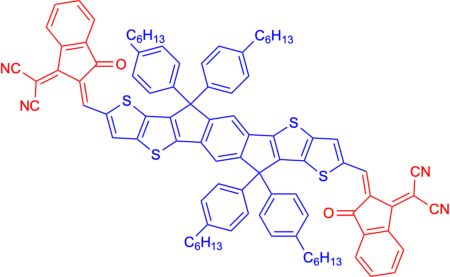
\includegraphics[width=0.6\linewidth]{images/ITIC.pdf}
    \caption{ITIC chemical structure with \textcolor{red}{electron accepting regions in red} and \textcolor{blue}{electron donating regions in blue}}
    \label{fig:itic}
\end{wrapfigure}

The planar acceptor-donor-acceptor moeity seen in many NFA backbones (see Figure \ref{fig:itic}) may have more efficient exciton splitting, as compared to a fullerene acceptor, at the heterojunction due to strong electronic coupling between the conjugated backbones of the NFA and the polymer\cite{Yi2018a}.

%%<how opvs work>
The compounds which compose an OPV are synthesizable molecules (often polymers) composed of abundant elements (carbon, hydrogen, nitrogen, sulfur, oxygen).
Due to the conjugated pi-orbitals in these molecules the absorption of sunlight can excite an electron into a frontier orbital and generate an exciton.
OPVs are made as a mixture of electron-donor and electron-acceptor compounds in a structure called a bulk-heterojunction.
Depending on the bulk morphology of these compounds, the exciton can travel to an acceptor-donor interface and dissociate into free electron and hole then these free charges generate current if they can subsequently make their way to an electrode.

%%<why morphology matters>
The morphology of the device can be affected by the processing conditions: temperature, solvents, and concentrations/ratios of the active compounds\cite{Ma2005,Hoppe2004a,Li2007}.
The interfacial area of the acceptor:donor regions\cite{Mazzio2015}, the regioregularity of the polymer\cite{Kim2006}, and electronic properties of the compounds\cite{Scharber2006a} all play an important role in the power conversion efficiency (PCE) of the device. 
These changes in structure can strongly affect the device performance.
Molecular simulation allows us to "see" these atomic interactions and gain a deeper view into the driving forces behind the self assembly of these OPV morphologies and to understand what conditions create the best devices.
%%<segue into simulation>

\subsection*{Molecular Dynamics}
%EJ: Here or above: Why MD the right tool?
Molecular dynamics (MD) is a simulation tool which uses classical physics and statistical thermodynamics to sample the equilibrium states of a thermodynamic ensemble.
The MD algorithm integrates Newton's equations of motion to update the particle positions.
This process can be iterated until the system reaches equilibrium.
MD is the right tool for looking at the bulk structure of an OPV because we can simultaneously probe the thermodynamics which govern OPV self assembly and the kinetics that follow the device processing.
Other tools, like Monte Carlo (MC), may allow us to sample equilibrium states of an ensemble, but we would lose information about the dynamics.
MC is also inefficient for polymers because perturbing a long chain of particles requires a "cluster move", which is not parallelizable.

%%<md in general>
MD separates the interactions between particles into non-bonded interactions and bond, angle, and dihedral interactions.
Non-bonded interactions are commonly modelled with a Lennard-Jones potential:
$$ U_{LJ}(r_{i,j}) = 4\epsilon\big[\big(\frac{\sigma}{r_{i,j}}\big)^{12}-\big(\frac{\sigma}{r_{i,j}}\big)^{6}\big]$$
Where $i$ and $j$ are the particles separated by distance $r_{i,j}$.
The equilibrium distance between particles is controlled by $\sigma$ and the depth of the potential well is controlled by $\epsilon$ (see Figure \ref{fig:lj}).
A distance cutoff, $r_{cut}$, is often used to reduce the number of pairwise interactions and improve performance.

\begin{wrapfigure}{L}{0.5\linewidth}
    \centering
    \includegraphics[width=0.6\linewidth]{images/lj.pdf}
    \caption{The Lennard-Jones potential with relevant distances labelled}
    \label{fig:lj}
\end{wrapfigure}

Particles connected by bonds are also modelled by classical forces, for example the bond potential may be treated as a harmonic oscillator:

\begin{wrapfigure}{L}{0.5\linewidth}
    \centering
    \includegraphics[width=0.4\linewidth]{images/bondangledihedral.pdf}
    \caption{Bonded interactions: bond (top left), angle (top right), and dihedral (bottom). Image adapted from \cite{punma}.}
    \label{fig:bad}
\end{wrapfigure}

$$V_{bond}(r) = \frac{1}{2}k(r-r_{0})^{2}$$
Where $r$ is the bond length, $r_{0}$ is the equilibrium bond length, and $k$ is the spring constant for the bond.
The angle potential is also treated as a harmonic oscillator:
$$V_{angle}(\theta)=\frac{1}{2}k(\theta-\theta_{0})^{2}$$
Where $\theta$ is the angle formed between three bonded particles, $\theta_{0}$ is the equilibrium angle, and $k$ is the spring contant for the angle.
The dihedral potential can be defined by the follow Fourier series:
$$V_{dihedral}(\phi)=\frac{1}{2}k_{1}(1-cos(\phi))+\frac{1}{2}k_{2}(1-cos(2\phi))+\frac{1}{2}k_{3}(1-cos(3\phi))\frac{1}{2}k_{4}(1-cos(4\phi))$$
Where $\phi$ is the angle between planes formed by particles in the dihedral (see Figure \ref{fig:bad}) and $k_{n}$ are the force coeffients.

%% transition???
The first MD simulation modelled a system of 108 particles and completed 200 collisions in one hour on an IBM-704\cite{Alder1957}.
Now GPUs are a 100 millions times faster.
%%<what is MD used for? why is MD the best technique for gettign these OPV morphologies?>
Due to its efficient scaling, MD is now commonly used for the modelling of protein folding \cite{levitt75} and other biological processes, and investigating the bulk properties of polymers\cite{Gartner2019a}.
By abstracting away some of the atomic degrees of freedom, MD can be used to look at even larger systems. %%transition attempt

%%<what assumptions does md make?>
Even all-atom MD is not without assumptions:
In general, during an MD simulation bonds aren't formed or broken, so without careful consideration this prevents the study of chemical reactions.
MD does not consider electrons, instead atoms are treated as point particles. 
This makes modelling systems which depend on hydrogen bonding or dispersion more difficult.

%%<what are the limits of atomistic md?>
Even with the simplifications of MD, we are still not able to simulate many systems efficiently on relevant length scales.
Therefore we can use a technique called coarse graining to increase the length and time scales we can examine.
%%<segue to why we need CG models>

\subsection*{Coarse Grain Models}

Coarse graining refers to grouping atoms in a structure into a "super-atom" and using an effective potential to represent the resulting coarse grain site.
Coarse grain models allow for simulators to access length and time scales that would be otherwise impossible using atomistic models by abstracting away irrelevant degrees of freedom.
%%<how do cg models let us access long length/time??>
Similarly to how we don't need to look at the working of a plant cell to understand the growth of a forest, we don't need to consider atomic level properties when we are interested in the bulk morphology\cite{Muller-Plathe2002}.
The heart of coarse graining is the removal of degrees of freedom. 
This effective potential used to represent the reduced system results in a smoothed free energy landscape. 
Processes which may have taken many time steps in an all atom simulation can take fewer time steps in a coarse simulation\cite{Berendsen2010}.
Due to their long length and time scales, coarse grain models are ideal for examining polymer properties\cite{Gartner2019a}.
It is too big and too slow and also just a bad idea to simulate huge boxes of atomistic polymers.
Even if the simulation was to complete, there would be too much information to process accurately. 
Coarse graining allows scientists to \textit{focus} their experiments\cite{Baschnagel2000}.

The resolution of coarse grain systems is broad:
Simply grouping hydrogens with the heavy atom they are bonded to, called the united-atom model, has been shown to speed up dynamics and make polymer length scales more easily accesible\cite{Paul1995a, Yang2006a}.
Other coarse-graining schemes may group functional groups together\cite{Berendsen2010, Jankowski2013, Marsh2014}, one bead per repeat unit in a polymer\cite{Lee2011}, or even represent an entire amino acid with a single site\cite{Peng2019}.
%%<examples of cg models and the cool things they do>
General coarse grain models of OPV thiophene polymers where only the spacing and regioregularity of the side chains were varied were able to predict order disorder transitions and scattering patterns comparable to those obtained from experiment\cite{Jankowski2013, Marsh2014}.
A coarse grain model for phospholipids has allowed for bilayer formation from an initial random configuration to be simulated even though the model was parameterized to the vapor-liquid phase transition\cite{Shelley2001}.
%% transition?
Which model is right depends on the length and time scale on which the property of interest can be observed.

%%<multiscale sims>
For many systems, however, we are interested in properties which span length scales.
For instance, in a system like a OPV polymer melt, it is not only computationally intractable to try and simulate the electron density on length scales proportional to the exciton dissociation length (~5-10 nm)\cite{Huang2010}; it is the wrong tool for the job.
If what we are interested in is the properties of the polymer in the bulk heterojunction, then it is wise to abstract away any degrees of freedom which do not directly contribute to the self-assembly of the structure.
Once a good bulk structure has been achieved, the atomistic details can be reintegrated much more easily: a process called backmapping.
In the same way that a coarse grain model can be mapped onto an atomistic one, we can get a reasonable starting structure for an atomistic simulation from a coarse grain structure.
The large length scale, polymer level properties can be equilibrated during the coarse grain simulation, and then the atomic interactions can be equilibrated during the backmapped atomistic simulation.
This can allow us the calculate properties such as charge transport, which depends upon the electronic structure of individual chromophores \textit{and} the connectivity of these chromophores over distances proportional to the exciton dissociation length.
%%<what stands in our way?>

%%<coarse-grain models are specific>

%%<segue from automated creation of forcefields to...>
%%<mapping operator has to be decided by hand> <is this section too big?>
Part of coarse graining that is not yet automated is choosing a mapping scheme or a mapping operator.
A mapping operator defines which atoms are grouped into a "super atom" represented by one coarse grain site and where the site is placed relative to the atom group.
Mapping operators are chosen based on the desired resolution of the coarse grain system and the information to be extracted.
A straightforward way to define a mapping operator is to group a set number of heavy atoms (non hydrogen) together; this is the method used in the MARTINI force field\cite{Marrink2007}.
In this scheme, four atoms (except rings, which are treated differently) are grouped and the site is classified as polar, non-polar, apolar, or charged depending on the atoms it is composed of.
When parameterizing a new molecule, you must pick a mapping and then compare the resulting beads to existing beads; a process which is time consuming and error prone\cite{martini-tutorial}.
%%The MARTINI force field was first designed for lipids, further parameterization for proteins and nuclei acids has since been added, and it has been shown to be effective in predicting vesicle formation, membrane protein dynamics, etc.%%<cite
Many other mapping schemes are simply based on the user's chemical intuition (e.g., what parts of the molecule shouldn't be allowed to bend? What groups have the most dominant interactions in this structure). %%<cite any model where rings are one bead><cite dna cg model>).
As the number of atoms in the fine grain structure increases, the number of possible mappings increase drastically.
There have been efforts to create algorithms for automating the process of deciding which atoms are grouped in a "super-atom" bead.
One study reduced the number of allowed mappings by only allowing those which do not change the symmetry group, then iterated over a graph of all possible mappings to find the "best" mapping by comparing the difference between the mapped RDF and velocity autocorrelation function\cite{Chakraborty2018b}.
Another uses principle component analysis to choose a mapping scheme for biomolecules that best represents th essential dynamics\cite{Zhang2008}.
Mapping operators can be automated using machine learning: clustering methods combined with graph analysis were shown to predict the "expert" mapping chosen using chemical intuition reliably\cite{Li2020}. 
A mapping operator based on the centers of charge was shown to accurately model electrostatic properties\cite{Cao2015a}.
%%<how cg potentials have been attained> 
Deciding on a mapping operator is one part of creating a coarse grain model, the second step is to create an effective potential for the site.

\subsection*{Multi-State Iterative Boltzmann Inversion}

There are numerous methods for deriving coarse grain potentials from atomistic ones (e.g., force-matching, reverse Monte Carlo), but in this proposal we will focus on Iterative Boltzmann Inversion (IBI).
%%<IBI>
IBI is where a coarse grain potential is iteratively tuned to fit a target distribution\cite{Reith2003}.
Here is the algorithm for determining the non-bonded potentials:
First the coarse grain system is mapped onto an equilibrated atomistic one.
Then the radial distribution function (RDF) of the mapped systems is calculated over the equilibrated frames of the trajectory--This is the target distribution.
Given any particle, the RDF gives the probability of finding a neighboring particle at distance r.
Taking the Boltzmann Inverse of the RDF results in the potential of mean force (PMF). %%<add equation>
%% equation
Then a CG simulation can be run using the PMF as the non-bonded potential to achieve a new distribution.
Then the difference between the new and target distribution can be accounted for in the next iteration accoring to equation %%<add equation>.
This process is repeated until the difference between the result and the target are sufficiently similar.

The coarse grain potential derived from IBI is not transferrable to different thermodynamic statepoints.
This is because the RDF is a property of the ensemble average at a given statepoint, so the potential derived from this property is also limited.
For example, separate potentials are required to capture solid and fluid structures of a pure simple lipid \cite{Hadley2010a}.
There are many attempts to create transferrable CG potentials, for example:
The TraPPE force-field fits CG potentials using vapor-liquid equilibria to improve transferrability across thermodynamic states\cite{Maerzke2011}.
But optimization to the liquid-vapor equilibrium, although useful for prediction of thermodynamic properties, may not be ideal for prediction of structure which will strongly influence charge transport.
%%<so we probably want to create our own potentials>
%%<IBI potentials are sometimes transferrable and it is not clear why sometimes they are and sometimes they aren't.> \cite{Moore2014}

Multistate iterative Boltzmann inversion (MS IBI) includes data from multiple targets to yield a less state dependent potential\cite{Moore2014}.
The MS IBI potential is an average of the single state potentials with a weighting function to prioritize a state of interest.
This method has been shown to accurately reproduce the true potential in monoatomic LJ fluid.

When using the MS IBI method, it is important to choose dissimilar states to minimize the potential overlap region.
If this overlap region is large, there are many potentials which will provide matching RDFs.

\begin{wrapfigure}{L}{0.5\linewidth}
    \centering
    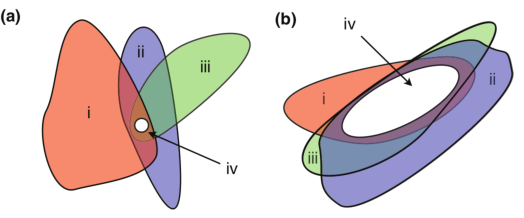
\includegraphics[width=0.6\linewidth]{images/moorefig.pdf}
    \caption{Visualization of the state space coverage of different potentials: if the thermodynamic states are too similar (b), then the overlap region is large enough that there are many potentials which will fit the target. Choosing states which are different (a) will better define the potential. Image taken from ref \cite{Moore2014}.}
    \label{fig:lj}
\end{wrapfigure}

For some systems there may not be a potential that represents all states; this is not unique to coarse potentials, atomistic potentials also have this limitation.
%%<need some tie in back to why we would want to go from CG-->atomistic>

\subsection*{Mesoscale Device Simulation}

%%<I DONT WANT TO FOCUS ON THIS TOO MUCH. It's only here as a rationale for why backmapping>
%%<how morphct pipeline would work: cg-backmap-ct>
MorphCT, a software previously developed by our lab, can simulate charge transport through an OPV morphology using kinetic Monte Carlo\cite{Miller2018a,MorphCT,morphct2.2}.
The kinetic Monte Carlo algorithm used by MorphCT uses the semi-empirical Zerner's Intermediate Neglect of Differential Overlap (ZINDO/S) quantum chemical calculation to obtain the molecular energy levels of chromophores in the morphology.
The HOMO levels of each chromophore site and the energy splitting induced in the chromophore pairs is used in the Marcus equation to calculate the charge hopping rate between pairs.
A Monte Carlo simulation can then be run using these hopping rates to calculate the movement of charges through the system.
Because this is a quantum chemical calculation, the position of each atom is needed; therefore, a backmapping process is required to calculate the charge transport in a coarse grain morphology.
%% MorphCT has some built in backmapping tools which use an xml file, but  (which i will discuss why these are bad in the next section) and the package is bulky/CLI/hard-to-use...
%%<making morphct more modular to allow it to be used in a workflow not cli>

\section*{Preliminary Work}

My prior work has involved probing the intermolecular interactions which govern dimer and crystal formation.
% With lan - About excitonic splitting, using DFT, DNA. 
An investigation of the excitonic splitting observed in cyanine dye dimers was done using density functional theory (DFT)\cite{Fothergill2018}.
By comparing calculated with experimental absorption spectra it was found that the solvent may play a large role in the dimer formation and peak shifting.
% With Matt - What intermolecular interactions guide diphenylurea crystal formation
An investigation of the supramolecular interactions which guide crystal self-assembly in diphenylurea transition metal complexes was done using density functional theory\cite{Millard2019a}. 
% With us - Perspective paper about all things
My contributions to our perspective paper were mostly about my experience joining the lab and trying to reproduce an existing model; a task which should be very straightforward in a computational field but which any computational scientist can attest is far from simple\cite{Jankowski2019}. 
 %% frame gixstapose as a tool for reproducible, approachable science
I also presented a tool I've developed, called GIXStapose, at the Scientific Python conference (SciPy2020). %%cite scipy and gixstapose
GIXStapose is an interactive structure viewer alongside its simulated diffraction pattern.
This work had two goals: helping users to see the connections between a structure and it's diffraction pattern and making reproducible figure generation easier.
The first goal is achieved through a graphical user interface (GUI) which allows users to interact with the structure using the mouse and the diffraction pattern is updated automatically.
The second goal is accomplished by allowing all steps of the figure generation process (e.g., positioning the camera, setting the colors and lighting, etc) to be scripted and never \textit{requiring} use of the GUI.
These prior works, although not directly related to OPVS or coarse grain models, have helped me think about how atomic interactions can shape a structure, the struggles that face a new computational scientist, and how I can help.

%%<how do I relate this to what I want to do??>
I have contributed to development of open-source packages including mbuild, foyer, signac, and fresnel. %%cite
These contributions have given me ample opportunity to excercise best software development practices like writing good documentation, using version control, writing unit tests, employing CI, using a fork \& pull workflow, etc.
This experience will help me to be more efficient in my future work.
I've also gained valuable experience as working as part of a team.
As I plan to integrate my future work with existing projects, good collaborative skills will be necessary.

%% experience teaching and creating material for people to learn
I have completed Software Carpentry training which has taught me how to break down complex ideas and give learners a chance to use their knowledge.
With these principles in mind, I have created tutorial examples to help current and future students understand scientific concepts and how to use computational tools. %% cite notebook examples
%%- started development on UFF repo for foyer.
%%This is an example of how to create a version controlled forcefield which can be automatically applied to a compound.
%%<atom typing is a pain and doing it manually is bad cite foyer paper>

As for work towards my proposed plan, I have created a minimum working example of a coarse-graining and backmapping package which uses SMARTS strings to specify the bead chemistries. %%cite grits
This package will need further testing as it is tested on different compounds, but the proof of concept exists.
%%<Talk about what exists and why it is not enough>
%%<votca, Peng2019a> 
Packages which do coarse-graining and backmapping already exist, so why is another one necessary?
One such package, Versatile Object-oriented Toolkit for Coarse-graining Applications (VOTCA)\cite{Ruhle2011b}, includes a coarse-graining, forcefield creation with reverse MC or IBI, and back-mapping modules.
It also allows for charge transport calculations using KMC similar to MorphCT\cite{Lukyanov2010}.
%%<compare VOTCA's backmapping to my proposed scheme>
VOTCA makes some progress towards a TRUE simulation pipeline: they include a docker container with their pre-built software stack and example input files.
However, some of these input files don't work and the unit test coverage on their examples repo at the of time of this writing is 0\%.
While including example inputs and a prebuilt software stack via docker is a great first step, these tutorials give very little walkthrough aside from code comments buried in the xml\cite{votca-github}.
A manual is provided but the example files and the explanation given in the manual is disconnected. %%cite <https://github.com/votca/csg-manual/releases>.
The code is a mix of C++, shell commands, and python, and the user is required to interact with compiled programs through the command-line which makes adding this code into an existing workflow a little more difficult.
And judging by the amount of confusion in their mailing list, there is room for improvement in the API.%% cite <https://groups.google.com/forum/\#!forum/votca>
Overall though this project has many features, interfaces with many popular MD engines (LAMMPS, GROMACS, HOOMD), and is under active, collaborative development, it is near-overwhelming in its scope and is not designed for the new user.
By choosing a pure python API I will be able to make use of Jupyter Notebooks which can be run on cloud servers using tools like MyBinder which can combine executable code with markdown text and images.%%<cite link mybinder, link to tutorials I;ve made>
In this way a tutorial can provide exact commands needed to reproduce the example intimately connected with the rationale and justification of that example.

For an example of what I mean by cognitive load, let's compare an example of my proposed coarse-graining scheme to VOTCAs.
In the following example we will take a hexane molecule and map it to three coarse grain sites (two carbon atoms per site).

\begin{wrapfigure}{L}{0.5\linewidth}
    \centering
    \includegraphics[width=0.6\linewidth]{images/hexane-compare.pdf}
    \caption{top: hexane chemical structure, bottom: hexane overlaid with coarse grain mapping \textcolor{blue}{A}-\textcolor{orange}{B}-}\textcolor{blue}{A}
    \label{fig:hexane}
\end{wrapfigure}

VOTCA uses an xml file to do this:

%%\lstinputlisting[breaklines]{hexane.xml}

\begin{wrapfigure}{L}{0.5\linewidth}
    \centering
    \includegraphics[width=0.6\linewidth]{images/hexanexml.pdf}
    \caption{XML file used by VOTCA to specify a three site coarse grain mapping of n-hexane}
    \label{fig:hexanexml}
\end{wrapfigure}

It may be easy to think that because the goal is simple, mapping two carbons and their attached hydrogens to a single bead so that six alkyl carbons becomes three coarse grain sites (A-B-A), that the process will also be simple.
In order to specify a bead-mapping using VOTCA, we need to know the residue number, the residue name, and the atom name.
For a six atom system this is not too bad, but it could get tedious and error-prone for larger systems.
And keep in mind that these xml files need to be created manually for each compound which is coarse grained or  backmapped.
VOTCA's scheme also requires that the bonding and the angles resulting from those bonds are specified, another process which is tedious, error-prone, and probably unecessary. 
To explain, let's discuss my proposed alternative:
\begin{lstlisting}
hexane_sites = [("_A", "C[CH3]"), ("_B", "CC")]
\end{lstlisting}
The result of using this code in the `coarse` function is a three-site hexane model A-B-A, same as VOTCA.%%<link to grits>
The mapping here is specified as a list of bead name SMARTS string pairs.
Although they do add some element of cognitive load, SMARTS strings are designed to be human and machine readable and can match atoms based on their chemical environment.
With this scheme, there is no need to look up the name or number of each residue, I simply specify that want two alkyl carbons (in SMARTS notation a capital "C" denotes an alkyl carbon) and requiring that one be a terminal carbon by including that it has three attached hydrogens ("[CH3]").
The order of the beads here matters because technically all the carbon atoms in hexane could be mapped with the more general SMARTS string (CC), so it is important to list the most specific strings first.
The bonding and angles of the resulting coarse grain beads can then inferred based on the bonding of the mapped atoms.
Basically what VOTCA's xml file does in 51 lines, I can do in 1 which is easier to read and makes chemical sense. 
There are even benefits to the mapping being inline with the code:
It allows the user to see the mapping as they progress through the workflow without having to search for multiple files.
Not using an external file may prevent common errors caused by manual file IO such as operating system specific line endings or whitespace characters like tab or space being read differently by a program.
Having the mapping in-line with the workflow also allows for the user to check that the mapping is correct with built in interactive visualizations, which can display the mapping as an overlay. 
(Figure \ref{hexane-compare} is the output of one such visualization using py3Dmol.) %%cite py3Dmol

We propose a way to make the mapping and backmapping process easier for the user.
Simplified Molecular Input Line Entry System or SMILES was designed to represent organic molecules in an unambiguous way (similar to IUPAC) but in a line-entry system which is also readable by a computer\cite{Weininger1988}.
This makes it a good candidate for specifying a coarse-grain mapping scheme.The open-source package, Openbabel, allows for a SMILES string to be converted to a chemical structure and vice versa.
SMARTS is similar to SMILES but instead of representing a single molecule unambiguously, it has multiple wildcards which can be used for pattern matching.%%<cite openbabel,SMILES, SMARTS>
This pattern matching is also implemented in the Openbabel package.
If we know the SMARTS string for any given CG mapping, we can map the CG site to its center of mass or geometric center.
I have developed a minimum working example of how this can be done and then how the atomistic structure can be recovered.%%<cite grits>
%% another application?
This mapping scheme could even be used to make the mapping process easier for established coarse grain models.
It could be fairly straightforward to implement a lookup to check if bead parameters already exist (e.g., for the MARTINI model) by going through and writing out the SMARTS pattern for each existing bead type.
This could make parameterizing new compounds for an existing method more foolproof.

\section*{Research Plan}

%% make better opvs
%% need to get a morphology on relevant lengthscale
%% many different chemistries
%% need a model that get a cg model from a chemistry

My plan is to create a workflow which builds on existing tools: signac, freud, mbuild, openbabel, and a previously developed msibi package.
This workflow could start with equilibrated atomistic trajectories from multiple statepoints, then use SMARTS strings to map the CG sites to each trajectory and calculate the effective potentials using MSIBI.
Once we have a tabulated coarse grain force field, we can create a larger simulation using our coarse grain model.
Finally, once we have an equilibrated coarse grain trajectory, we can using backmapping to regain the atomic positions and do analysese such as radial distribution function (RDF), charge transport, and diffraction.
If this workflow is streamlined, it can be applied to many different compounds allowing for a high-throughput analysis of many potential OPV compounds.

%% Objectives are like steps along the way
%% objectives should be
% 1. goal of the step
% 2. how to do the step
% how doing this achieves the goal
%% how to coarse grain reproducibly
\subsection*{Objective 1: Develop a generalized toolset for coarse graining and performing simulations of novel molecules for organic photovoltaics}
% mapping
% ff creation
% infrastructure: porting ff to engine
In order to model the morphologies of new OPV chemistries, we need a simple way to generate novel coarse grain models.
This objective consists of three steps:
\begin{enumerate}
    \item {Create a tool that uses a mapping operator to go from atomistic to coarse grain structure}
    \item {Use the mapped coarse grain structure to parameterize a force field using MSIBI}
    \item {Develop the infrastructure to port this force field to a simulation engine}
\end{enumerate}
A minimum working example of this coarse grain mapping tool has been completed. %% cite grits, cg-tutorial
However, it will still need to be tested with many more compounds and mapping operators.
This package uses the chemical file format parsing and scriptable structure building capabilities of mbuild coupled with the SMARTS/SMILES string matching of the openbabel package to generate coarse grain structures mapped onto their atomistic counterparts with only a SMARTS string from the user.
These coarse grain structures mapped to an atomistic target can then be used in an MSIBI workflow to obtain an effective potential.
A minimum working example of an MSIBI tool has also been started; %https://bitbucket.org/cmelab/msibi_tests/src/master/ do i even mention this?
although the hands-on experience with MSIBI was useful to me in getting a better understanding for the process, I think for future, I will build off an existing MSIBI code. %%https://github.com/mosdef-hub/msibi
The force field obtained using MSIBI will then be used to run a simulation of a novel coarse grain model.
Therefore decisions about how to carry the forcefield information into a simulation engine will need to be made.
Here we will focus on HOOMD, but transferrability among simulation engines will be a goal.
The coarse graining workflow will be considered complete when it can be used to coarse grain a test set of 25 common OPV chemistried. % 25 is just in there as a random number
% workflow is complete when we can cg these chemistries
% use ff in different sim engines

\subsection*{Objective 2: Develop a general tool to retrieve atomistic information from a coarse grain morphology}

In order to calculate the charge transport of a coarse grain OPV system, we need to be able to regain the atomic positions.
Given an equilibrated coarse grain trajectory, we can reintroduce the atomistic degrees of freedom by using the same SMARTS mappings used for coarse graining.
The chemistries specified by the SMARTS strings will be mapped onto the centers of the CG sites and then equilibrated in a short MD run using the atomistic force field with an additional position restraint to maintain the structure. 
I have developed a minimum working example of this backmapping process, %% cite grits
however, the specification of how the backmapped atomistic structures are bonded is still not intuitive for the user to specify and I am not sure yet how to make it better.
The backmapping workflow will be considered complete when it can backmap a test set of 25 common OPV chemistries from all possible mappings.

\subsection*{Objective 3: Predict nanostructure of novel OPV chemistries}

Once Objectives 1 and 2 are complete, the next step will be putting them to use to investigate new OPV compounds.
Currently, I have not found CG models for many NFA compounds (e.g, ITIC). %% I found this paper \cite{Meng2019} that claims to do CGMD with PTB7 ITIC but the details are hidden in the SI and seem fishy. seems like they use IBI but they dont say how they got their target distributions.
A simple, useable coarse graining tool will be helpful for determining the best mapping operator to use for these OPV compounds.
To help organize the dataspace of the large parameter sweep, I plan to use the signac package to manage an ever-changing workspace.
This will help easily and efficiently test out different mappings and "processing" conditions.

% predict nanostructure of new opv blends TODO new objective?
% do math -- how long will it take me to graduate? how many sims can i do?

\subsection*{Objective 4: Analysis} % calulcate mobilities compare structural properties to experiment
% identify chemical features correlated to robust mobilities

Our lab has shown that we have the capability to compare our simulation results to experiment using hole mobilities from charge transport calculations\cite{Jones2017,Miller2018a} and grazing incedent X-ray scattering (GIXS) patterns\cite{Miller2018}.
GIXS calculations on our backmapped trajectories can be used to validate that our simulations result in the same morphology as experiment.
While charge transport calculations can be used to rate the efficacy of the active layer morphology.
Using our lab's charge transport package (MorphCT) on new chemistries, however, will require some work.
Many of the parameters and the definition of the chromophore are hard-coded for poly-3-hexylthiophene (P3HT).
Moving this package away from a command line interface will also be a goal of this work.
%%Our morphct paper says the mobilities we predict are 2x higher than experiment? why?
%%<I need something in here about making morphct more user friendly and less hard-coded for p3ht.>
%%<adding in calculation of reorganization energy??> 
%%<or just ripping out the KMC bit and making it modular>

\section*{Predicted Outcomes}

As a result of this work, we expect the following outcomes:

\begin{enumerate}
    \item {\textbf{Gain insight into the limits of coarse-graining}}
        This work will probe the limits of coarse graining to understand the minimal model necessary to represent different OPV chemistries.
    \item {\textbf{Understand the interactions which guide BHJ self assembly}} 
        This work will test a variety of different OPV compounds. 
        Comparing the results may provide understanding into which moeities, intermolecular interactions, or processing conditions result in the morphology with the highest charge transport.
    \item {\textbf{Understand the mapping operator}}
        This work will test whether using a chemical string format (SMARTS/SMILES) to specify the atomistic to coarse grain site mapping is a viable alternative to other methods. 
        Using SMARTS/SMILES strings allows a user to more easily and intuitively specify a mapping.
        If specifying a mapping is easier, a user may be more willing to try out a greater number of different mappings.
        This would allow for the comparison of a system parameterized with different mapping operators.
    \item {\textbf{Benefits of Transferrable, Reproducible, Usable, Extensible research}} %%what am i trying to say here?
        Does making science easier/more understandable make it better? %more reproducible? curb cuts
        If parameterizing a coarse grain force field is easier and more approachable, it would open up more possibilities for trying different mapping schemes or different structural or thermodynamic targets rather than sticking to an existing force field.
        Better coarse grain models could result in more accurate and efficient simulation of large length scale systems.
\end{enumerate}

\section*{Contingency Analysis}

%%<what's going to be hard?> 
Although minimum working examples have been developed for botht the coarse graining and backmapping packages, I still expect to struggle when mapping new compounds.
Sometimes the SMARTS/SMILES mapping won't work without careful choice of beads.
This can be a little frustrating but is still preferrable to having to manually specify the mapping of each atom.
At least the reasons that a SMARTS mapping fails are usually understandable (e.g., the order of the beads matters) or chemically sensible (e.g., one SMILES string may contain another -- just as one chemical moeity may be composed of more submoeities). %%<this is a word?>)

It may also be difficult to find a good coarse graining scheme for the NFA compounds. 
These compounds are often composed of large planar backbones with floppy side chains.
Finding a suitable mapping to represent both aspects may be difficult.

\section*{Timeline for Implementation and Evaluation}
\begin{table}[h]
    \resizebox{\columnwidth}{!}{
%\resizebox{\textwidth}{!}
    %\centering
    \renewcommand{\arraystretch}{1.1}
    \begin{tabular}{| c | c | c | c | c | c | c | c | c | c | c | c | c | c | c | c | c | c | c | c | c |}
        \hline
        \multirow{2}{*}{PROJECT TASK}& \multicolumn{4}{c}{YEAR 1} &  \multicolumn{4}{|c}{YEAR 2} & \multicolumn{4}{|c}{YEAR 3} & \multicolumn{4}{|c|}{YEAR 4} & \multicolumn{4}{c|}{YEAR 5} \\ 
        \hhline{~--------------------}
             & 1  & 2  & 3  & 4  & 1  & 2  & 3  & 4  & 1  & 2  & 3  & 4  & 1  & 2  & 3  & 4 & 1  & 2  & 3  & 4\\
        \hline
           Complete Coursework & \multicolumn{10}{|c|}{ {\cellcolor{lgray}} } &  &  &  &  &  &  &  &  &  &\\
        \hline
           Present at a Conference  &  &  &  &  &  &  &  &  &  &  & x &  &  &  &  &  &  &  &  &\\
        \hline
           Publish a First Author Paper  &  &  &  &  &  & x  &  &  &  &  &  &  &  &  &  &  &  &  &  &\\
        \hline
           Proposal and Comprehensive Exam  &  &  &  &  &  &  &  &  &  &  &  & * &  &  &  &  &  &  &  &\\
        \hline
           Expand Functionality of Open Source Packages & & & & & & \multicolumn{11}{|c|}{{\cellcolor{lgray}}} & & & &\\
        \hline
           Develop Coarse Graining Package              & & & & & & & & & \multicolumn{8}{|c|}{{\cellcolor{lgray}}} & & & &\\
        \hline
           Develop Automated MS-IBI Code                & & & & & & & & & \multicolumn{8}{|c|}{{\cellcolor{lgray}}} & & & &\\
        \hline
           Develop Backmapping Package                  & & & & & & & & & & & & \multicolumn{5}{|c|}{{\cellcolor{lgray}}}& & & &\\
        \hline
           Generate Coarse-Grain Morphologies           & & & & & & & & & & & & & & \multicolumn{4}{|c|}{{\cellcolor{lgray}}}& & &\\
        \hline
           Evaluate OPV Device Performance & & & & & & & & & & & & & & \multicolumn{4}{|c|}{{\cellcolor{lgray}}} & & &\\
        \hline
           Write Dissertation & & & & & & & & & & & & & & & &{\cellcolor{lgray}}& {\cellcolor{lgray}}& {\cellcolor{lgray}} &  &\\
        \hline
           Present Dissertation Defense  &  &  &  &  &  &  &  &  &  &  &  &  &  &  &  &&  & {\cellcolor{lgray}} &  &\\
        \hline
             %Saved row template
             %&  &  &  &  &  &  &  &  &  &  &  &  &  &  &  &  \\
    \end{tabular}}
    \caption{Anticipated timeline. * indicates right now, X indicates already accomplished.}
\end{table}
